\documentclass[10pt]{article}

\usepackage[top=0.4in, bottom=0.4in, left=0.6in, right=0.6in]{geometry}
\usepackage{tikz}
\usetikzlibrary{positioning}
\usepackage{enumitem}
\usepackage{graphicx}
\usepackage{tgheros}
\renewcommand*{\familydefault}{\sfdefault}

\setlength{\parskip}{0pt}

% Change this value to resize the grade circle on the quiz header.
\newlength{\gradeCircleRadius}
\setlength{\gradeCircleRadius}{0.35in}

% Set this to the letter identifying this quiz version (e.g. A, B).
\newcommand{\quizVersion}{B}

% Reference diagram of the flash memory map, shown above Question 2 to help
% students locate the bootloader and application regions and their vector
% tables (not to scale).
\newcommand{\flashMapDiagram}{%
\begin{center}
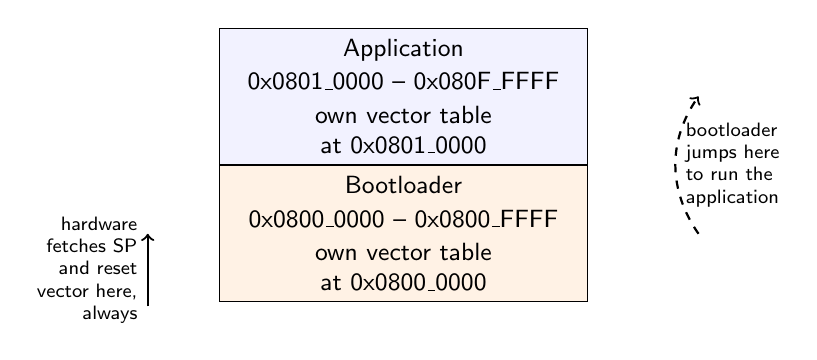
\begin{tikzpicture}[region/.style={draw, align=center, font=\small, text width=4.4cm, inner sep=4pt}]
\node[region, minimum height=1.6cm, fill=blue!5] (app) {Application\\[1pt] 0x0801\_0000 -- 0x080F\_FFFF\\[1pt] own vector table at 0x0801\_0000};
\node[region, minimum height=1.0cm, fill=orange!10, below=0pt of app] (boot) {Bootloader\\[1pt] 0x0800\_0000 -- 0x0800\_FFFF\\[1pt] own vector table at 0x0800\_0000};
\draw[->, thick] ([xshift=-0.9cm]boot.south west) ++(0,-0.05) -- node[left, font=\scriptsize, align=right] {hardware\\fetches SP\\and reset\\vector here,\\always} ([xshift=-0.9cm]boot.west);
\draw[->, thick, dashed] ([xshift=1.4cm]boot.east) to[bend left=35] node[right, font=\scriptsize, align=left] {bootloader\\jumps here\\to run the\\application} ([xshift=1.4cm]app.east);
\end{tikzpicture}
\end{center}}

% Lays out four multiple-choice answers in a compact 2x2 grid.
\newcommand{\mcfour}[4]{%
\begin{center}
\begin{tabular}{@{}p{0.47\linewidth}@{\hspace{0.04\linewidth}}p{0.47\linewidth}@{}}
#1 & #2 \\[3pt]
#3 & #4 \\
\end{tabular}
\end{center}}

\pagestyle{empty}

\begin{document}

\noindent
\begin{minipage}[t]{\dimexpr\textwidth-2\gradeCircleRadius-0.5in\relax}
    {\large\textbf{ECGR 4101/5101 --- Advanced Embedded Systems}}\par
    \textbf{Quiz 2: Startup Process and Bootloaders --- Version \quizVersion}\\[8pt]
    Name: \makebox[2in]{\hrulefill} \quad Date: \makebox[1.1in]{\hrulefill}
\end{minipage}%
\hfill
\raisebox{0.15in}{%
\begin{minipage}[t]{\dimexpr 2\gradeCircleRadius+0.2in\relax}
    \centering
    
\begin{tikzpicture}[baseline=(circtop.base)]
        \coordinate (circtop) at (0,\gradeCircleRadius);
        \draw[very thick] (0,0) circle (\gradeCircleRadius);
        \draw[very thick] ({\gradeCircleRadius*cos(225)},{\gradeCircleRadius*sin(225)}) -- ({\gradeCircleRadius*cos(45)},{\gradeCircleRadius*sin(45)});
        \node at ({0.36*\gradeCircleRadius},{-0.4*\gradeCircleRadius}) {\Large\textbf{10}};
    \end{tikzpicture}
\end{minipage}}

\vspace{0.05in}
\textit{For each question, circle the letter of the correct answer.}

\vspace{0.05in}

\setlist[enumerate]{topsep=0pt, itemsep=2pt, parsep=0pt}

\begin{enumerate}[label=\textbf{\arabic*.}, leftmargin=*, itemsep=3pt]

\item \textbf{(5 points)} There is no operating system on a bare-metal microcontroller to set up memory before your code runs -- the microcontroller's own startup code has to do that job itself.

\begin{enumerate}[label=(\alph*), leftmargin=*, itemsep=3pt]
\item \textbf{(2 points)} Which of the following correctly orders the sequence of events that take place on a generic Cortex-M microcontroller between power-up and the execution of the first instruction in \texttt{main()}?

\begin{center}
\begin{tabular}{@{}rl@{}}
\textbf{(A)} & SP load $\rightarrow$ reset-vector load $\rightarrow$ \texttt{.bss} zero $\rightarrow$ \texttt{.data} copy $\rightarrow$ early setup $\rightarrow$ \texttt{main()} \\
\textbf{(B)} & early setup $\rightarrow$ SP load $\rightarrow$ reset-vector load $\rightarrow$ \texttt{.data} copy $\rightarrow$ \texttt{.bss} zero $\rightarrow$ \texttt{main()} \\
\textbf{(C)} & SP load $\rightarrow$ reset-vector load $\rightarrow$ early setup $\rightarrow$ \texttt{.data} copy $\rightarrow$ \texttt{.bss} zero $\rightarrow$ \texttt{main()} \\
\textbf{(D)} & reset-vector load $\rightarrow$ SP load $\rightarrow$ early setup $\rightarrow$ \texttt{.data} copy $\rightarrow$ \texttt{.bss} zero $\rightarrow$ \texttt{main()} \\
\end{tabular}
\end{center}

\item \textbf{(2 points)} A global variable is declared \texttt{int calOffset = 7;}. If the startup code's copy of the \texttt{.data} section from flash into SRAM were skipped, what value would \texttt{calOffset} actually have the first time \texttt{main()} reads it?

\mcfour{\textbf{(A)} Garbage already sitting in SRAM}{\textbf{(B)} 7 (baked into the machine code)}{\textbf{(C)} 0 (SRAM defaults to zero)}{\textbf{(D)} The program fails to compile}

\item \textbf{(1 point)} A global variable is declared \texttt{static int errorFlag;} with no explicit initializer. If the \texttt{.bss} zero-initialization step were skipped at startup, what value would \texttt{errorFlag} have the first time \texttt{main()} reads it?

\mcfour{\textbf{(A)} 7, same as \texttt{calOffset}}{\textbf{(B)} 0 (C guarantees it, no hardware needed)}{\textbf{(C)} The program fails to compile}{\textbf{(D)} Garbage already sitting in SRAM}
\end{enumerate}

\item \textbf{(5 points)} A bootloader and the application it manages are built as two separate programs that share one physical flash chip, as shown below (addresses are representative, not to scale).

\vspace{-4pt}
\flashMapDiagram
\vspace{-6pt}

\begin{enumerate}[label=(\alph*), leftmargin=*, itemsep=3pt]
\item \textbf{(1 point)} At reset, hardware always fetches the initial stack pointer and reset vector from the same fixed base address of flash (0x0800\_0000 above). Based on this, which program must be placed at that fixed address?

\mcfour{\textbf{(A)} The bootloader}{\textbf{(B)} The application}{\textbf{(C)} A separate ``reset program''}{\textbf{(D)} Either one -- it does not matter}

\item \textbf{(2 points)} The bootloader jumps to the application's reset handler without ever changing the processor's vector-table pointer. Immediately afterward, an interrupt fires. Whose interrupt handler actually executes?

\mcfour{\textbf{(A)} The application's}{\textbf{(B)} Whichever is closest in flash}{\textbf{(C)} Neither -- a hard fault, no handler at all}{\textbf{(D)} The bootloader's}

\item \textbf{(1 point)} What is the one action the application's startup code must take so that interrupts are correctly routed to its own handlers instead of the bootloader's?

\mcfour{\textbf{(A)} Move the application's code to 0x0800\_0000}{\textbf{(B)} Disable all interrupts permanently}{\textbf{(C)} Update the vector-table pointer to the application's own table}{\textbf{(D)} Recompile the bootloader without a vector table}

\item \textbf{(1 point)} Why must the bootloader and application be built as two separate projects, each with its own linker script defining a non-overlapping flash region?

\mcfour{\textbf{(A)} It is not required -- only a style preference}{\textbf{(B)} So each can be (re)flashed independently}{\textbf{(C)} They would otherwise be forced to share one stack pointer}{\textbf{(D)} One linker script cannot produce more than one vector table}
\end{enumerate}

\end{enumerate}

\end{document}
